\documentclass[tikz,border=1cm]{standalone}
\definecolor{lightgreen}{RGB}{198,239,206}
\definecolor{darkgreen}{RGB}{45,125,51}
\usepackage{kpfonts}
\usepackage{lipsum}
\usepackage{tabularray}
\usetikzlibrary{calc,positioning,arrows.meta}
\tikzset{corner/.style={font=\sffamily,text=darkgreen,scale=.8}}
\newcommand{\zjrpic}[8][]{%
    \node[text=darkgreen,font=\sffamily\bfseries,draw,fill=lightgreen,align=center,minimum width=4cm,minimum height=2cm,#1] (#2) {#3\\[5pt]#4};
    \node[anchor=north,corner]
    at ($(#2.north west)!0.3!(#2.north)$) (#2-LU) {#5};
    \node[anchor=north,corner]
    at ($(#2.north east)!0.3!(#2.north)$) (#2-RU) {#6};
    \node[anchor=south,corner]
    at ($(#2.south west)!0.3!(#2.south)$) (#2-LD) {#7};
    \node[anchor=south,corner]
    at ($(#2.south east)!0.3!(#2.south)$) (#2-RD) {#8};
}
\begin{document}

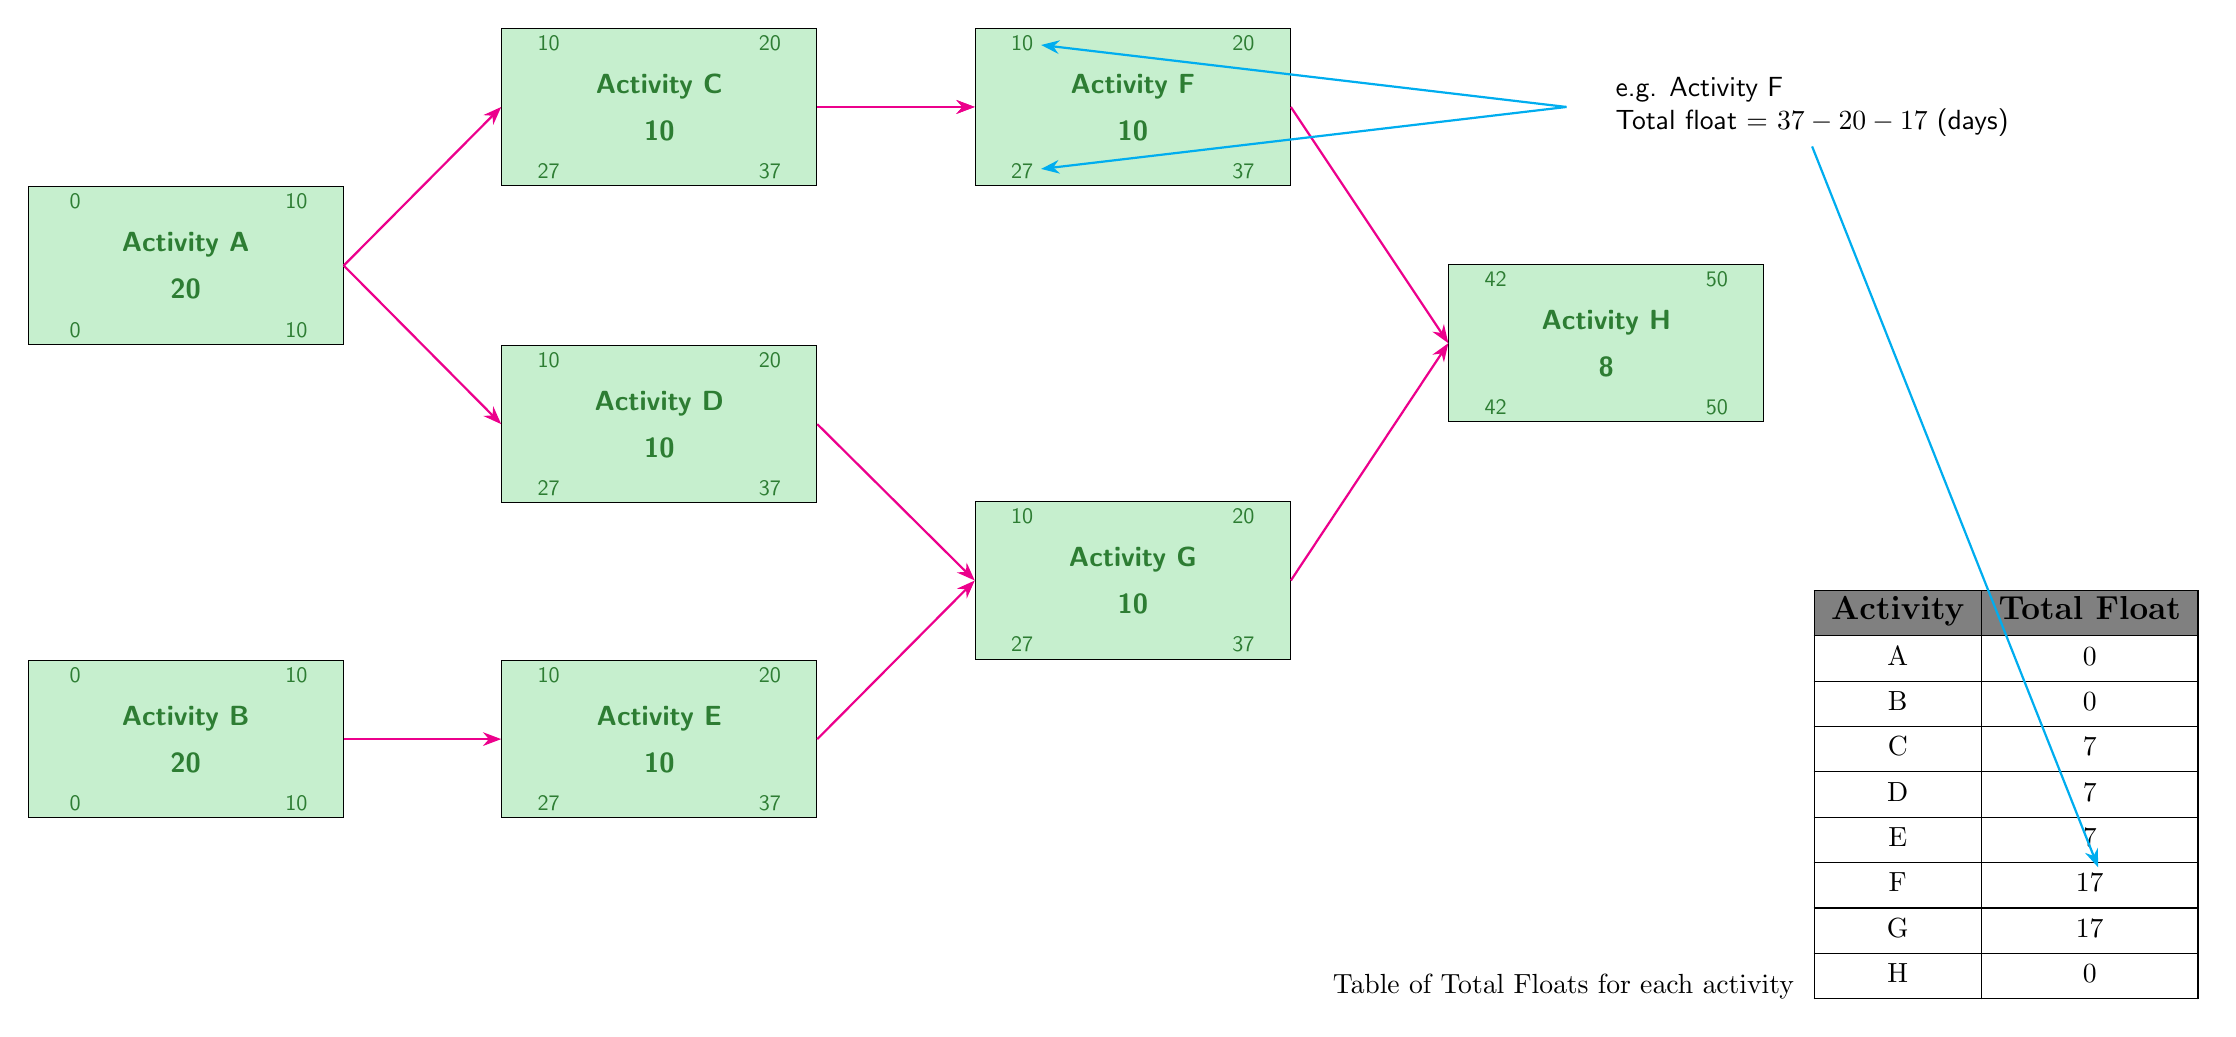
\begin{tikzpicture}[>=Stealth]
    \zjrpic{A}{Activity A}{20}{0}{10}{0}{10}
    \zjrpic[below = 4cm of A]{B}{Activity B}{20}{0}{10}{0}{10}
    \zjrpic[above right = 0cm and 2cm of A]{C}{Activity C}{10}{10}{20}{27}{37}
    \zjrpic[below right = 0cm and 2cm of A]{D}{Activity D}{10}{10}{20}{27}{37}
    \zjrpic[right = 2cm of B]{E}{Activity E}{10}{10}{20}{27}{37}
    \zjrpic[right = 2cm of C]{F}{Activity F}{10}{10}{20}{27}{37}
    \zjrpic[above right =0cm and 2cm of E]{G}{Activity G}{10}{10}{20}{27}{37}
    \zjrpic[above right =1cm and 2cm of G]{H}{Activity H}{8}{42}{50}{42}{50}
    \path[magenta,thick]
        foreach \i/\j in {A/C,A/D,B/E,C/F,D/G,E/G,C/F,F/H,G/H} { (\i.east) edge[->] (\j.west)}
    ;
    \node[right=4cm of F,align=left,font=\sffamily] (example) {e.g. Activity F\\Total float = $37-20-17$ (days)};
    \draw[cyan,->,thick] ([xshift=-.5cm]example.west) -- ([xshift=.5cm]F-LU);
    \draw[cyan,->,thick] ([xshift=-.5cm]example.west) -- ([xshift=.5cm]F-LD);
    \node[below right=2cm and .5cm of H] (tblr) {
        \begin{tblr}{
            colspec={*{2}{Q[c,m]}},hlines,vlines,
            row{1}={font=\bfseries\large,gray},
        }
            Activity & Total Float \\
            A & 0 \\
            B & 0 \\
            C & 7 \\
            D & 7 \\
            E & 7 \\
            F & 17 \\
            G & 17 \\
            H & 0 \\
        \end{tblr}
    };
    \coordinate (tblr-mark) at ([xshift=-1.4cm,yshift=1.8cm]tblr.south east); % ugly with absolute coordinate...
    \draw[cyan,->,thick] (example.south) -- (tblr-mark);
    \node[left=0cm of tblr.south west,anchor=south east] {Table of Total Floats for each activity};
\end{tikzpicture}%

\end{document}